\documentclass[10pt]{ps-exercise}
\usepackage{float}
\author{Raphael Gwiggner and Christoph Sch\"opf}
\date{\today}
\subject{Distributed Systems}
\title{Sheet 02}

\begin{document}
\section{Protocol}
\begin{quote}
a) All required messages: \\ \\
Client:
\begin{itemize}
\item Username
\item "1" for Addition
\item "2" for Subtraction
\item "3" for Multiplication
\item "4" for Factorial
\item 1. Operand
\item 2. Operand (is 0 for Factorial)
\end{itemize}
Server:
\begin{itemize}
\item Login succesful?
\item Result
\end{itemize}
b) format of messages
\begin{itemize}
	\item Username : String - only sends one string to the server
	\item Service data : [Operation : Int, Operand1 : Int, Operand2 : Int] - on the client side an array of length 3 represents the data for the service. At index 0 is the operation, at index 1 is the first operand and at index 2 is the second operand. Tue to the table of operations \\
	\begin{tabular}{l | l}
	1 & Addition \\
	2 & Subtraction \\
	3 & Multiplication \\
	4 & Factorial
	\end{tabular}\\
	client and server know which integer indicates which operation. 

\item Login successful : boolean - tells the client if the login was successfully. 
\item Result : Int - the result of the operation is always one singe integer. 
\end{itemize}
\end{quote}
\begin{figure}[H]
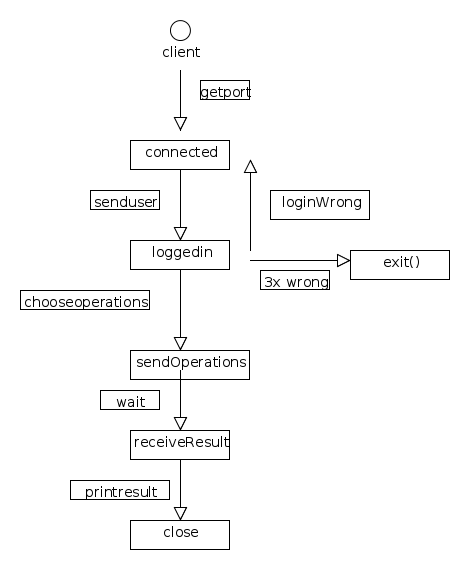
\includegraphics[scale=0.6]{client.png}
\end{figure}
\begin{figure}[H]
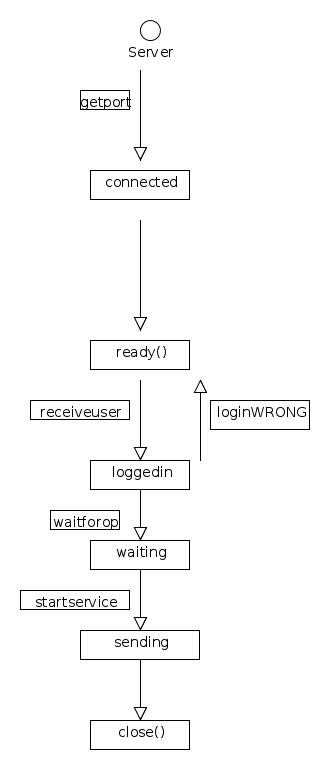
\includegraphics[scale=0.6]{server.png}
\end{figure}
\end{document}